\documentclass{report}
\usepackage{graphicx}
\usepackage{authblk}
\usepackage{amsmath}
\usepackage{listings}
\usepackage{subfigure}
\usepackage{algorithm2e}
\usepackage{minted}
\usepackage{booktabs}
\usepackage{float}
\usepackage{enumitem}
\usepackage{multirow}
\usepackage{diagbox}
\usepackage{subfigure}
\usepackage{pgfplots}


\title{ME 489\\ Homework 5 - MPI Implementation of Explicit In-time Two-Dimensional Finite Difference Solver}

\author{Ata Bora Çakmakcı}
\author{Mustafa Yiğit Görgün}

\affil{Middle East Technical University}
\date{7 January 2024}

\begin{document}
\maketitle
\tableofcontents
\chapter{Introduction}
In this study we parallelized an explicit in-time, two-dimensional, finite
difference solver using MPI. The wave equation to be solved by the already provided solver is as shown.
$$
\frac{\partial^2 q}{\partial t^2}=c^2\left(\frac{\partial^2 q}{\partial x^2}+\frac{\partial^2 q}{\partial y^2}\right), 0 \leq x \leq 1,0 \leq y \leq 1
$$
The equation is discretized utilizing second-order finite-difference method to approximate the value of the field variable \emph{q} at the next time step.
$$
q_{i, j}^{n+1}=2 q_{i, j}^n-q_{i, j}^{n-1}+\alpha_x\left(q_{i+1, j}^n-2 q_{i, j}^n+q_{i-1, j}^n\right)+\alpha_j\left(q_{i, j+1}^n-2 q_{i, j}^n+q_{i, j-1}^n\right)
$$

Where the next value of \emph{q} is determined by using its current, past and neighbouring values. An example solution at the last time step with trivial values is shown in Figure \ref{fig:1020_10}.
\begin{figure}[h]
    \centering
    \includegraphics[height=5in,width=5in,angle=0]{figures/MPI_1020_10.png}
    \caption{Post processed solution at the last time step for a problem size of 1020*1020}
    \label{fig:1020_10}
\end{figure}
\chapter{Implementation}
\section{MPI Implementations}
To start with we included the MPI header and initialized MPI. The rank and size of processes are obtained.
\section{Domain Decomposition}
Since we are instructed to assume the number of nodes in the Y direction is divisible by MPI size, we start off with dividing total number of nodes in Y direction to the MPI size and storing it as the local number of nodes in the Y direction.
When computing the coordinates of the nodes we need to make sure that y-coordinates of the nodes has to be unique to the process. To ensure that we made the following adjustment to the computation of coordinates.
\begin{minted}{c}
double yn = ymin + j*hy + rank*ny*hy;
\end{minted}

\section{Communication Between Processes}
We included two halo rows in allocating memory to the \emph{q} values. This allows us to create a space where the process can store the received value. Inside the solver we use MPI\_Send and MPI\_Recv to communicate the top and bottom most real row of values to the upper and lower processes respectively. We are also allocating memory for global values for $q^{n-1}$, $q^{n}$, \emph{x} and \emph{y}. These memories are to be filled with values coming from all processes to be printed in the rank 0. In order to collect the values from every process and fill in these global values we used MPI\_Allgather. Global values are necessary for printing out the values for checking the results while halo rows necessary for calculations.

\section{\emph{applyBC} Function}
Since this function is writen in only considering the series case it needed some adjustment. We changed the function such that it only applies boundary condition to the bottom-most row when rank=0 and to the top-most row when rank=size-1. The boundary condition loop for left and right is unchanged.

\section{Solver}
Since we implemented the halo rows, the solver isn't ignoring boundary rows correctly. The only rows that are ignored are the halo rows. Hence we are going to reapply the boundary conditions after the second-order finite-difference part to correct this mistake in the first and the "size"th process. 

\section{Printing Results}
In all of the sections where some form of results is to be printed in either the screen or a file we made sure that only one of the processes print out the results by using the global variables we mentioned before.
We also recorded the time elapsed using MPI\_Wtime() function for each of the processes. We then use MPI\_Reduce to get the one with the maximum value then print it as our wall time elapsed in seconds.

\chapter{Results and Discussion}
\section{Results}
The post processing of the evolution of the solution throughout the time steps and the solutions at the last time step at different resolutions can be seen in Figure \ref{fig:180_evo} and Figure \ref{fig:res_evo} respectively.
\begin{figure}[h]
\begin{center}
\subfigure[]{\includegraphics[height=1.5in,width=1.5in,angle=0]{figures/MPI_180_0.png}}
\subfigure[]{\includegraphics[height=1.5in,width=1.5in,angle=0]{figures/MPI_180_5.png}}
\subfigure[]{\includegraphics[height=1.5in,width=1.5in,angle=0]{figures/MPI_180_10.png}}
\caption{Evolution of the solution for 180*180 resolution at (a)0 (b)0.5 and (c)1 seconds}
\label{fig:180_evo}
\end{center}
\end{figure}
\begin{figure}[h]
\begin{center}
\subfigure[]{\includegraphics[height=1.8in,width=1.8in,angle=0]{figures/MPI_20_10.png}}
\subfigure[]{\includegraphics[height=1.8in,width=1.8in,angle=0]{figures/MPI_60_10.png}}
\subfigure[]{\includegraphics[height=2.2in,width=2.2in,angle=0]{figures/MPI_180_10.png}}
\subfigure[]{\includegraphics[height=1.8in,width=1.8in,angle=0]{figures/MPI_1020_10.png}}
\caption{Post process of the solution at the last time step for (a) 20*20 (b)60*60 (c)180*180 and (d)1020*1020 resolutions with same parameters}
\label{fig:res_evo}
\end{center}
\end{figure}

\pagebreak
Firstly, we recorded the time elapsed for different number of MPI processes with different resolutions. Then we plotted the time elapsed versus number of MPI processes for 180*180 resolution to make a strong scaling analysis. We also ran the code multiple times to get an average value for the time elapsed.
\begin{table}[h]
    \centering
    \hspace*{-2cm}\begin{tabular}{|c|c|c|c|c|c|c|}
        \hline
        \diagbox[width=13em, height=5em]{Resolution}{Number of Processes} & series & 1(with MPI) & 2 & 4 & 6 & 10\\
        \hline
        20*20 & 0.309022 &0.419144 & 0.241538 & 0.155123 & 0.200903 & 0.155488 \\
        \hline
        60*60 & 2.558143 &2.930173 & 1.622076 & 0.914772 & 1.028260 & 0.780037 \\
        \hline
        180*180 & 23.115470 & 24.243686 & 12.603723 & 7.178683 & 6.844577 & 5.659869 \\
        \hline
    \end{tabular}
    \caption{Elapsed time(s) for different number of processes with different problem sizes.}
    \label{table1}
\end{table}
\newpage
\begin{table}[H]
    \centering
    \begin{tabular}{|c|c|c|c|c|c|}
        \hline
        \diagbox[width=13em, height=5em]{Resolution}{Number of Processes}  & 2 & 4 &6 &10\\
        \hline
        20*20  & 0.640 & 0.498 &0.256 & 0.199\\
        \hline
        60*60  & 0.789 & 0.699 &0.415 & 0.328\\
        \hline
        180*180  & 0.917 & 0.805 & 0.563 & 0.408\\
        \hline
    \end{tabular}
    \label{table2}
    \caption{Scaling factors of parallelization with MPI with respect to the serial version of the code}
\end{table}





\begin{figure}[H]
  \centering
  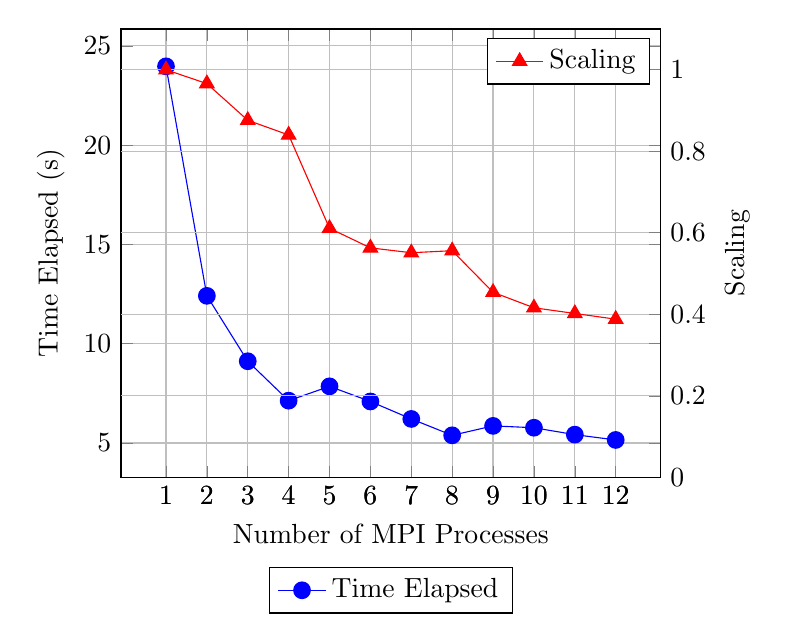
\begin{tikzpicture}
    \begin{axis}[
      xlabel={Number of MPI Processes},
      ylabel={Time Elapsed (s)},
      legend style={at={(0.5,-0.2)},anchor=north},
      xtick={1,2,...,12},
      grid=major,
      mark size=3,
      ]
      \addplot[blue,mark=*] coordinates {
        (1, 23.965352)
        (2, 12.408444)
        (3, 9.114984)
        (4, 7.128962)
        (5, 7.850184)
        (6, 7.088842)
        (7, 6.209419)
        (8, 5.384149)
        (9, 5.859639)
        (10, 5.766582)
        (11, 5.418631)
        (12, 5.151165)
      };
      \addlegendentry{Time Elapsed}

    \end{axis}
    \begin{axis}[
      axis y line*=right,
      ylabel near ticks,
      ylabel={Scaling},
      xtick={1,2,...,12},
      ytick={0,0.2,0.4,0.6,0.8,1.0},
      ymajorgrids=true,
      yminorgrids=true,
      ymin=0,
      ymax=1.1,
      mark size=3,
      ]
      \addplot[red,mark=triangle*] coordinates {
        (1, 1.0)
        (2, 0.966)
        (3, 0.876)
        (4, 0.840)
        (5, 0.611)
        (6, 0.563)
        (7, 0.551)
        (8, 0.556)
        (9, 0.454)
        (10, 0.416)
        (11, 0.402)
        (12, 0.388)
      };
      \addlegendentry{Scaling}
    \end{axis}
  \end{tikzpicture}
  \caption{Time Elapsed and Scaling vs. Number of MPI Processes for a problem size of approximately 180*180}
  \label{fig:mpi_time_scaling_graph}
\end{figure}



\newpage
\section{Discussion}
\paragraph{}
The first thing observed about this study is solely implementing MPI into the code without actually utilizing it results in worse performance than series version which makes sense but it can be seen from the Table \ref{table1} the difference in series version and 1 process version continues to increase while percent-wise decrease. This can be due to the initializing of MPI and the time it takes depends only on the problem size. In Table \ref{table1} this statement proves to be correct since the time differences are increasing with multiply of 3 while the problem size in Y direction is also increasing with a multiply of 3.
\paragraph{}
Secondly it can be seen from the \ref{table2} that as the problem size gets smaller implementing MPI yields less increase in performance. This is due to the above mentioned situation where MPI takes a certain ammount of time to run depending on the problem size in the Y direction. As the problem size gets bigger and bigger the time taken by the solver increases more rapidly than the time taken by the MPI hence the effect of the time taken by the MPI in the scaling decreases revealing a more accurate scaling of the implementation.
\paragraph{}
Finally it can be seen from the Figure \ref{fig:mpi_time_scaling_graph} that in MPI implementation time elapsed decreases as the number of processes increases up to 5 processes. At the 5 process we observe a jump in the behaviour of the time elapsed and this point also points out the dip of the scaling factor too. It can be said that as long as the scaling is concerned this solver should be run with at most 4 processors. On the contrary, if the time is an issue, the solver can be run with 12 or more processors.
\end{document}